\chapter{QCD Multijet Background: The Rebalance and Smear Method}
\label{chap:qcd}

The third and final background of the \mttwo analysis arises from mis-measured
jets in QCD multijet events (and, to a much lesser degree, in events with 
hadronically-decaying top quarks or vector bosons). 
This background is greatly suppressed by the
\mttwo and \dphimet cuts and hence is the smallest of the three backgrounds. 
However, it is also the most difficult to model and estimate since it depends
strongly on the peculiarities of the CMS detector and its imperfect response to jets.

QCD Monte Carlo cannot be relied upon to model this correctly (and statistics are too poor
anyway, due to the high cross section and low acceptance), so a data-driven technique is required.
This iteration of the analysis employs a new ``Rebalance and Smear'' method 
to estimate the multijet background. We briefly describe the old method and reasons 
for switching, then explain in detail the new technique.

\section{The $\Delta\phi$-ratio method}

Previous iterations of this analysis \cite{CMS:mt22016,CMS:mt22015} 
used the ``$\Delta\phi$-ratio'' method to estimate QCD background.
The method utilizes the variable $\dpmin \equiv \dphimet$ defined in
Sec.~\ref{sec:objvardefs}. Events with a badly measured jet tend to have
small \dpmin, as a single mis-measured jet drives the \vMet. Consequently,
inverting the $\dpmin>0.3$ requirement in the signal regions gives a 
conrol region enriched in QCD multijet events.

The $\Delta\phi$-ratio method estimates multijet contribution to the 
signal region by scaling events in this low-\dpmin control region
by a transfer factor $r_\phi(\mttwo) = N(\dpmin > 0.3) / N(\dpmin < 0.3)$.
Note that the numerator is ``signal region-like'' (\vMet far from any jets),
while the denominator is ``background-like'' (\vMet close to a jet).
From simulation, the functional form of this ratio as a function of \mttwo
is found to be well-described by a power law,
\be
r_\phi(\mttwo) = \frac{N(\dpmin > 0.3)}{N(\dpmin < 0.3)} = a\cdot\mttwo^b,
\ee
for sufficientyly high \mttwo. Below $\mttwo\approx60$ \GeV, the power law
form breaks down as the dominant source of \vMet is not from jet mismeasurement
(e.g. energy from pileup may contribute more significantly).

This ratio is measured in data in a low-\mttwo sideband, 
with an upper bound of $\mttwo=100$ \GeV.
Above this, the contribution from electroweak processes (\ttjets and V+jets)
is too high relative to QCD to allow an accurate measurement. The lower bound
is 60 \GeV for $\Ht<1200$ \GeV, and 70 \GeV for $\Ht\geq1200$ \GeV. Data for the measurement
is taken from pure-\Ht triggers (prescaled for $\Ht<1200$ \GeV). The fit is done inclusively
in \njets and \nbtags, and in the same \Ht bins as the main analysis. Fig.~\ref{fig:rphi}
shows example fits for 2017 data in the medium and high \Ht regions.

\begin{figure}
  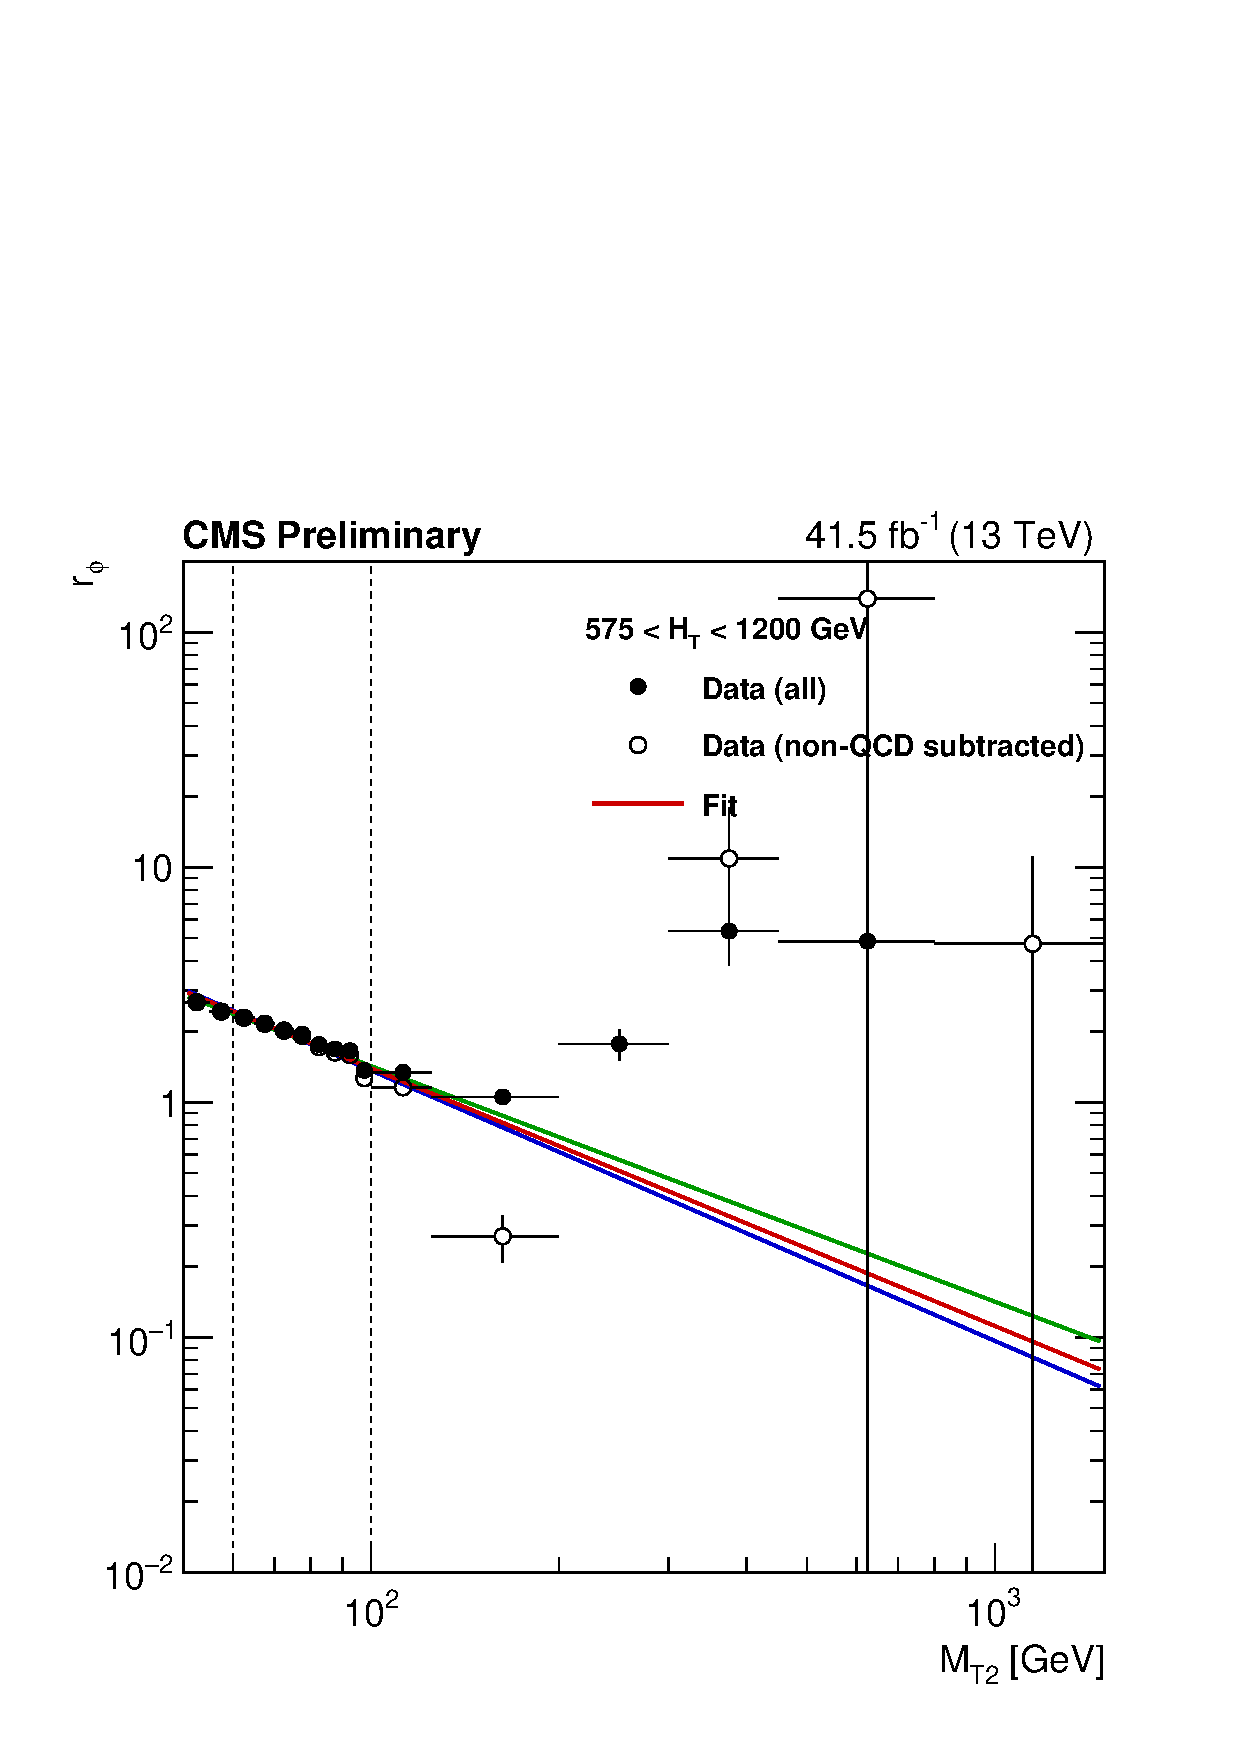
\includegraphics[width=0.48\linewidth]{figs/qcd/rphi_data_ht575to1200.pdf}
  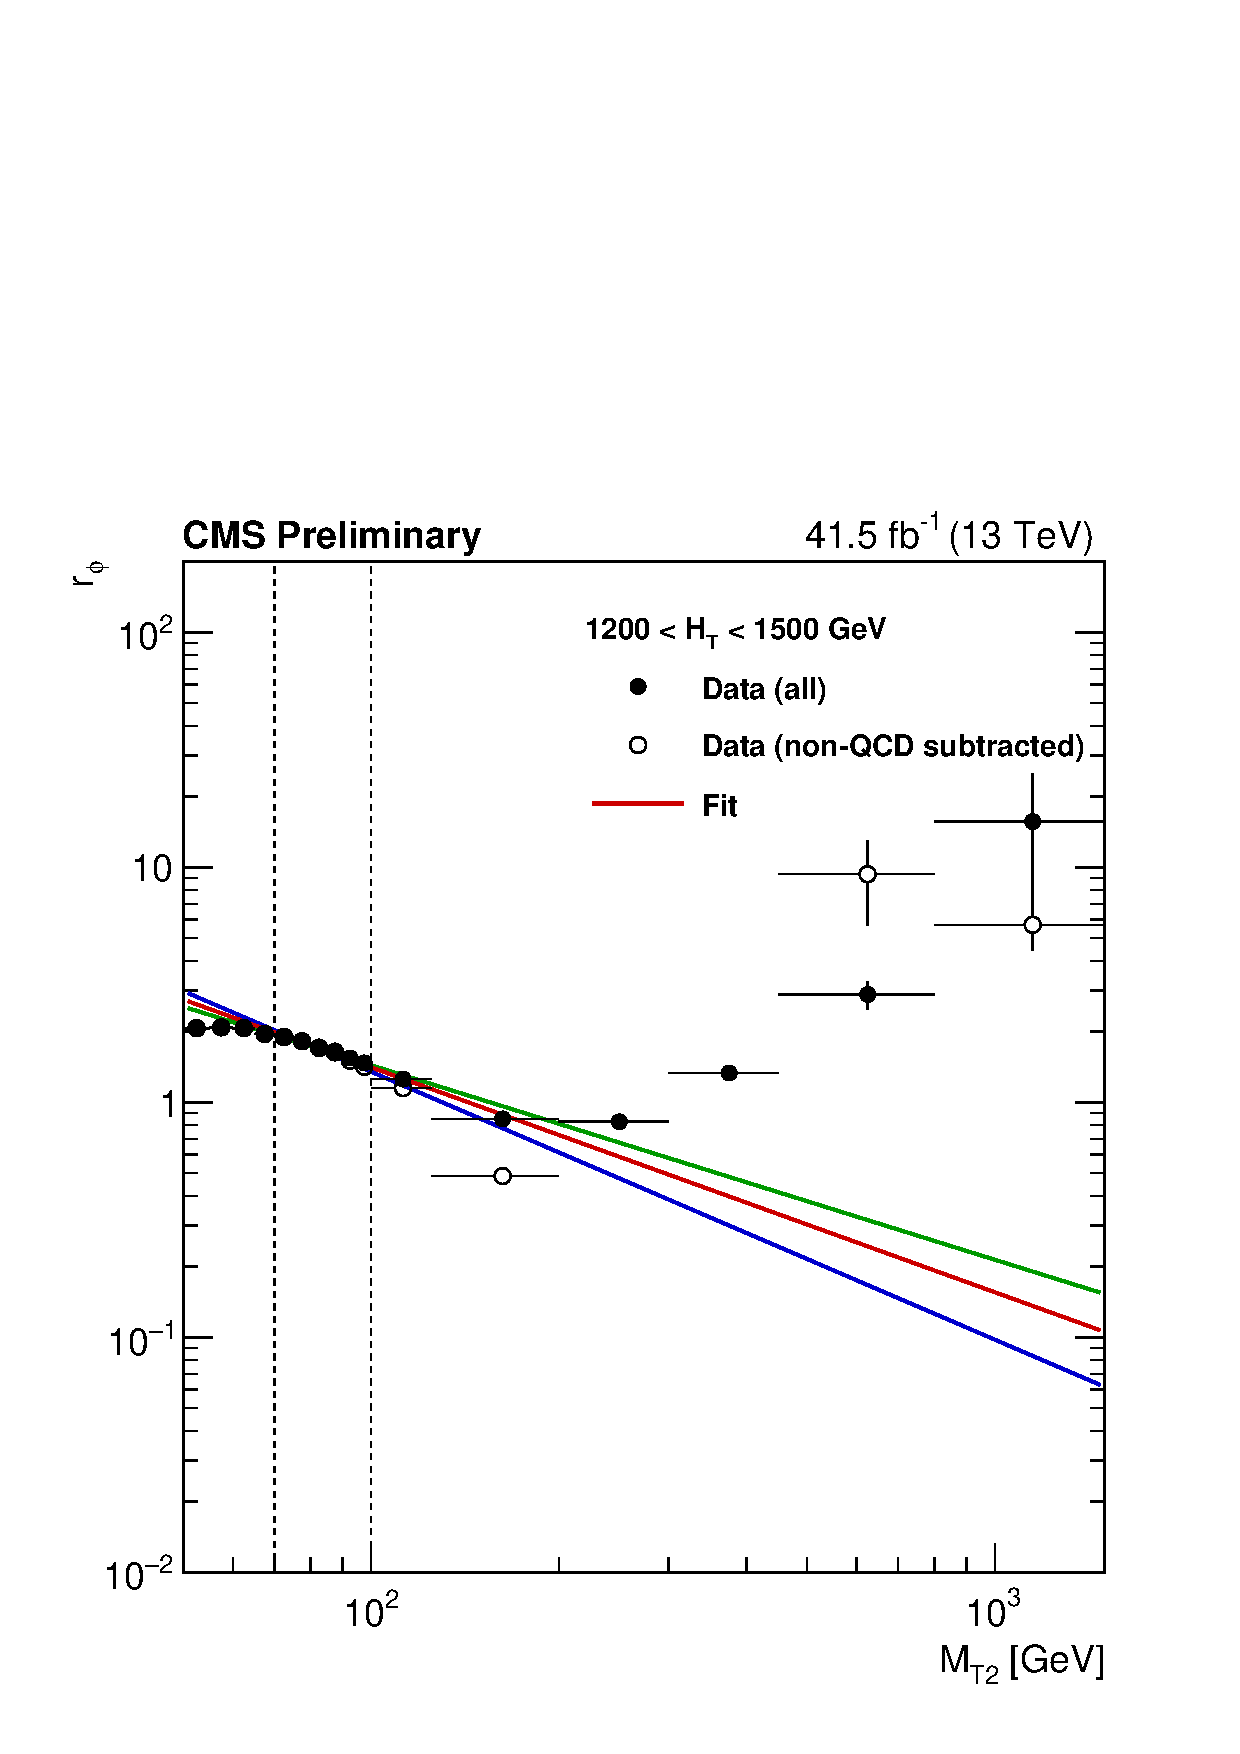
\includegraphics[width=0.48\linewidth]{figs/qcd/rphi_data_ht1200to1500.pdf}
  \caption{Example measurements of $r_\phi(\mttwo)$ in 2017 data, 
    for the medium and high \Ht regions. Black points are straight from data;
    white points have contribution from electroweak MC subtracted off from 
    both the numerator and denominator. Vertical dashed lines show the fit region.
    The red line is the central fit; the green and blue lines show the variations
    from extending the fit window one bin on the low or high edge, respectively.}
  \label{fig:rphi}
\end{figure}

\begin{figure}
  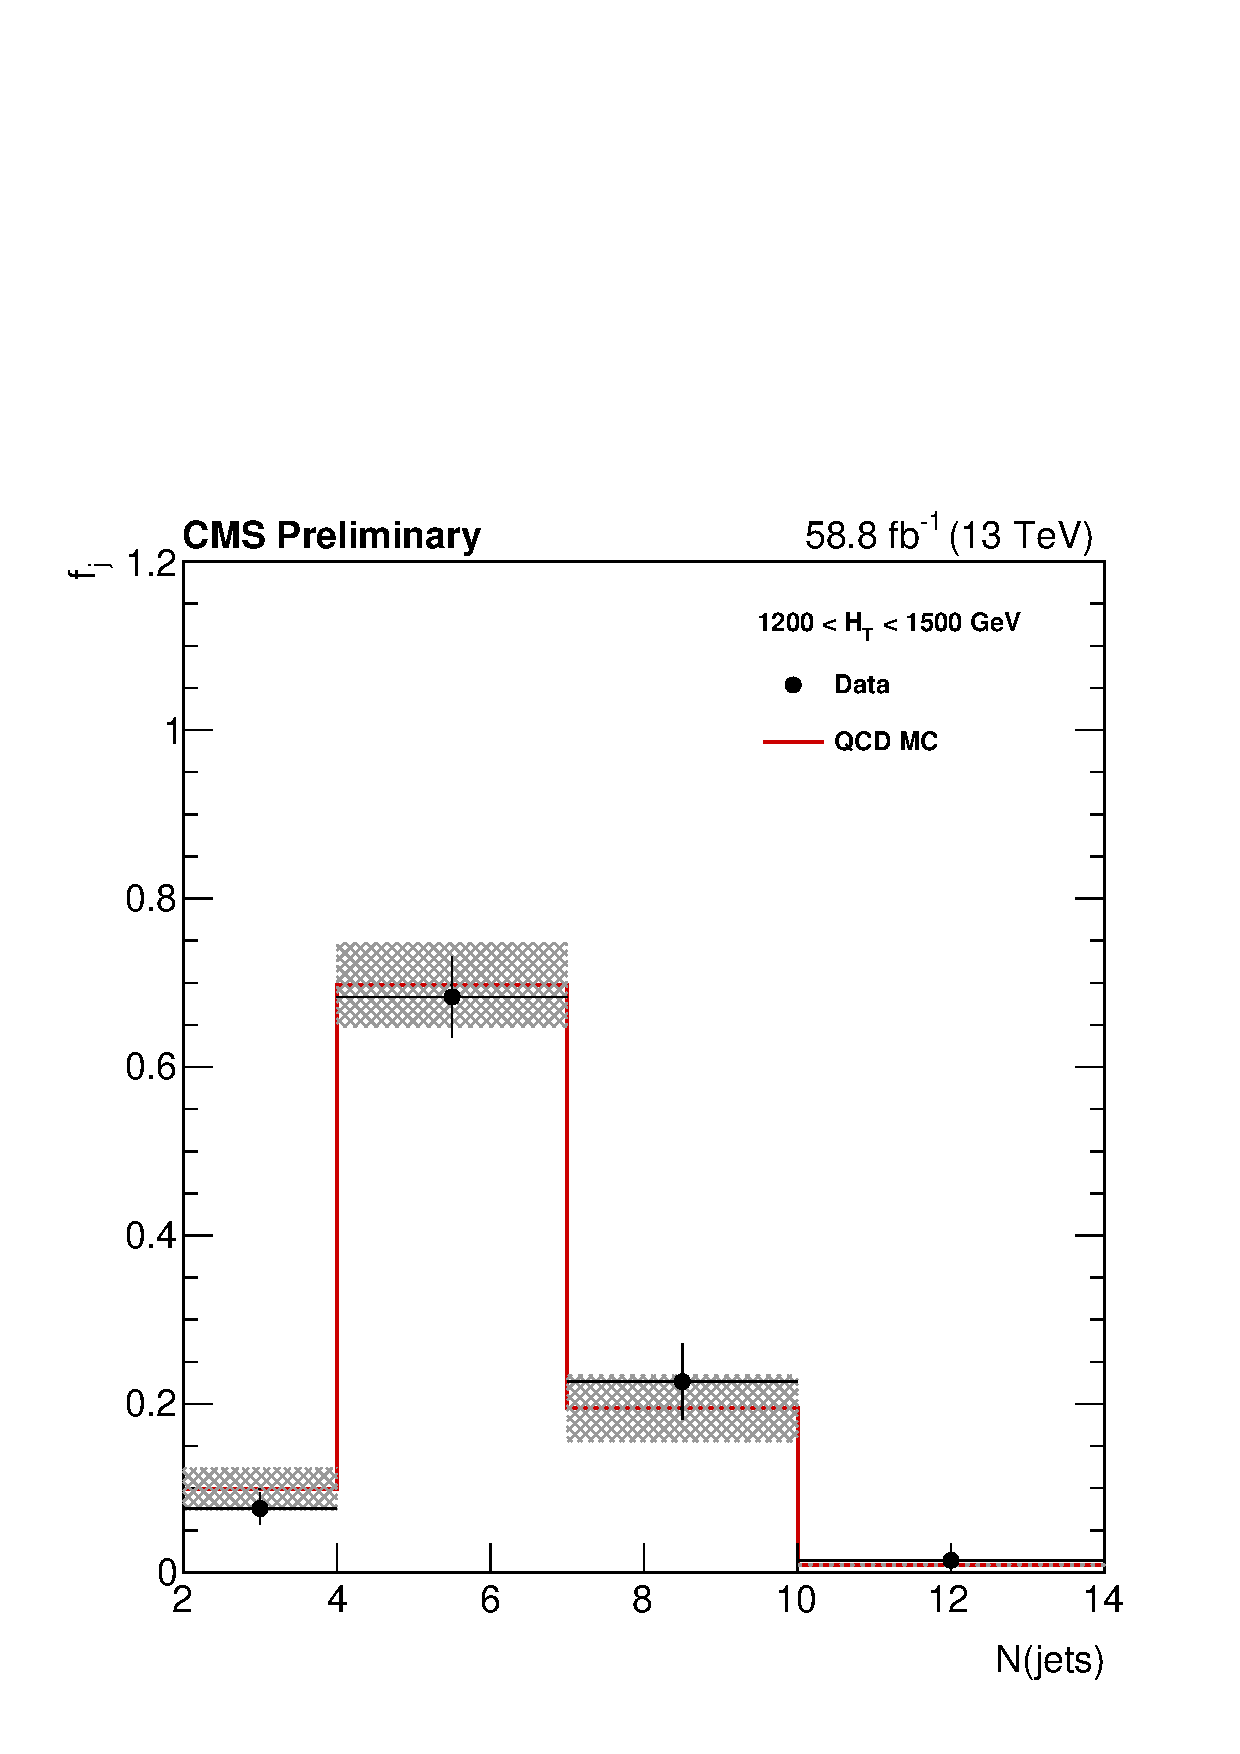
\includegraphics[width=0.48\linewidth]{figs/qcd/fj_ht1200to1500.pdf}
  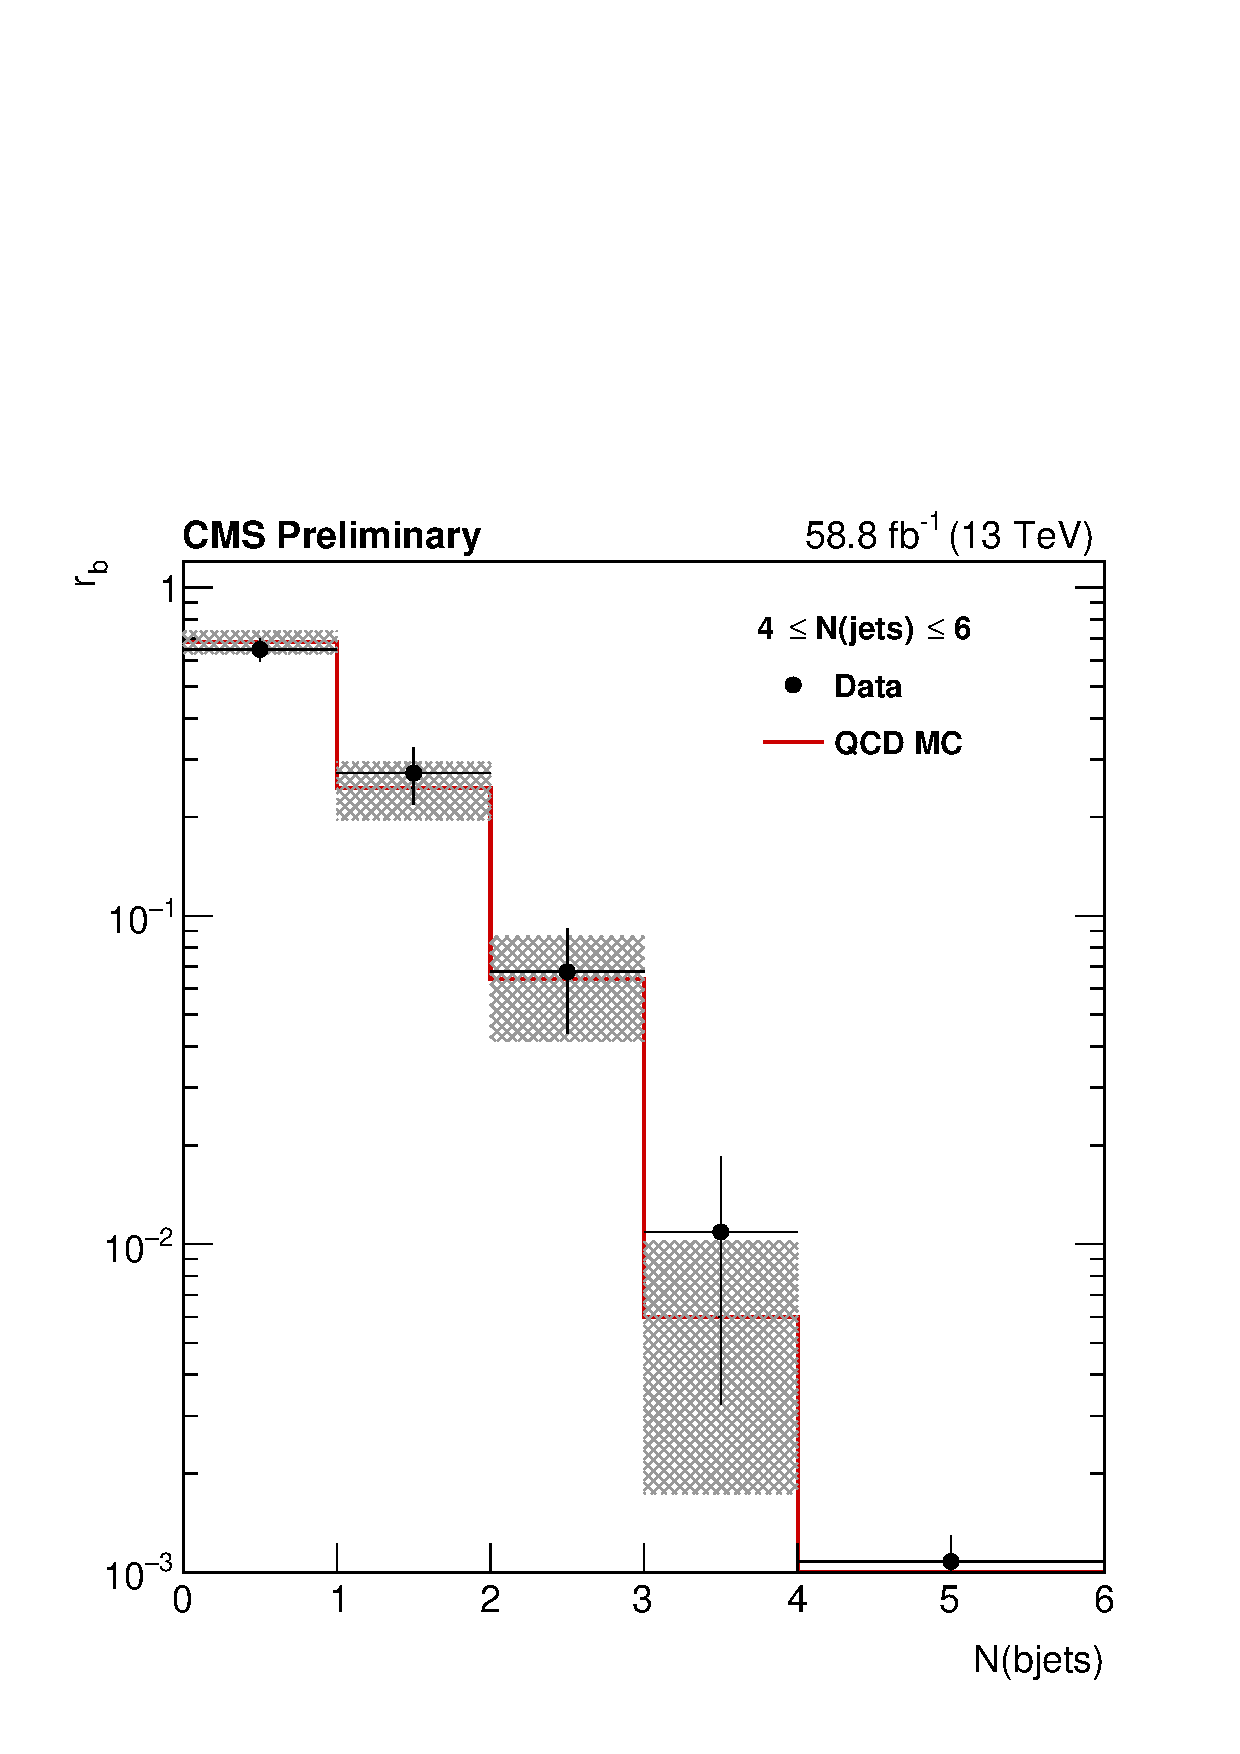
\includegraphics[width=0.48\linewidth]{figs/qcd/rb_j4to6.pdf}
  \caption{Transfer factors $f_j$ (left) and $r_b$ (right) measured in 2018 data. $f_j$
    is shown for $1200\leq\Ht<1500$ \GeV, and $r_b$ is shown for $4\leq\njets\leq6$.
    Data agrees with simulation within the uncertainties.
}
  \label{fig:fjrb}
\end{figure}

Each event in the low-\dpmin control region (integrated across \njets and \nbtags)
 is weighted by $r_\phi(\mttwo)$ to get its contribution to the signal region.
It remains to distribute events among the \njets and \nbtags bins. This is done through
transfer factors $f_j$ and $r_b$. The first, $f_j$ is the fraction of events falling into a particular
\njets bin, and the second, $r_b$, is the fraction of events in a given \njets bin falling into a particular
\nbtags bin. It is found through simulation that both $f_j$ and $r_b$ 
are invariant with respect to $\mttwo$, and $r_b$ is invariant with respect to \Ht.
It is further found that the shapes are equivalent at $\dpmin < 0.3$ and $\dpmin >0.3$.
These facts allow us to measure $f_j$ and $r_b$ in a QCD-enriched control region ($\dpmin<0.3$,
$100 < \mttwo < 200$ \GeV), $f_j$ in bins of \Ht and $r_b$ in bins of \njets.
Example measurements of $f_j$ and $r_b$ in 2018 data are shown in Fig.~\ref{fig:fjrb}.

Once all three of $r_\phi$, $f_j$, and $r_b$ are measured, we can get a final
signal region estimate as
\be
N_\mrm{SR}(\Ht,\njets,\nbtags,\mttwo) = \left(\sum_{\dpmin<0.3} r_\phi(\mttwo) \right) \cdot f_j(\Ht) \cdot r_b(\njets),
\ee
where the sum is taken over all events in a given \Ht region, inclusively in \njets and \nbtags.

\section{Overview of Rebalance and Smear}

While the $\Delta\phi$-ratio method has been used as the primary multijet estimation technique
in the past, there are a number of motivations to look for a better, more robust method.
Most importantly, the $\Delta\phi$-ratio method relies on a fairly severe extrapolation 
($r_\phi$ is measured in $60 < \mttwo < 100$ \GeV, and is used to predict signal region 
yields at $\mttwo>200$ \GeV), with no way to explicitly check its validity in the 
region of interest. Moreover, the power law fit function itself is emperically derived
from simulation, with no underlying theoretical motivation that would give one confidence
in its applicability.

An alternate method that is used as the primary multijet estimation technique in this 
iteration of the analysis is known as Rebalance and Smear (\rs).
The method consists of two distinct steps. The first, ``rebalancing'', seeks to adjust
the \pt of jets in multijet events such that the resulting \ptmiss is approximately zero,
with the aim of reproducing the true hard-scatter event which has no \ptmiss.
This is performed through a likelihood maximization, accounting for jet energy resolution.
The output of the rebalancing is an inclusive sample of multijet events with approximately
zero \ptmiss that are used as a seed for the second step, the ``smearing''. In this step, the
\pt values of the rebalanced jets are smeared according to jet response functions, in order
to model the instrumental effects that lead to nonzero \ptmiss. The smearing step is repeated many
times for each rebalanced event, which allows the accumulation of events in the tails
of kinematic distributions such as \ptmiss and \mttwo and for a more precise estimate 
of the multijet background in the signal regions.

Both the rebalancing and smearing steps make use of ``jet response templates'', which are distributions
of the ratio of reconstructed jet \pt to generator-level jet \pt. The templates are derived from simulation
in bins of jet \pt and $\eta$, separately for b-tagged and non-b-tagged jets. Details on the deriviation
of the templates are given in Sec.~\ref{sec:jrt}.

For \rs in data, events from pure-\Ht triggers are used. Events with $\Ht<1200~\GeV$ come
from prescaled triggers, and get weighted by the corresponding event-level prescale value in the final
prediction.

In addition to the trigger selections, events must contain at least one good vertex, two jets
with $\pt>10~\GeV$, and pass the standard event cleaning filters in order to be used in the \rs.
No other selections are applied.

\subsection{Rebalancing}
The rebalancing procedure adjusts the \pt of jets in an event with the aim of reproducing the true
hard-scatter event which has no \ptmiss. Note that only the magnitude of the jet \pt is modified,
while the jet direction remains unchanged.

Of all jets in the event, a jet qualifies for use in the rebalancing and smearing procedure if it has $\pt>10$\GeV,
and if it is not identified as a jet from pileup in the case that $\pt<100$\GeV.
All other jets are left unchanged but are still used in the calculation of \vMet and other jet-related quantities.
An event with $n$ qualifying jets is rebalanced by varying the $p_\text{T}^\text{reb}$ of each jet to maximize the likelihood function
\be
\label{eq:rebalance_likelihood}
L = \prod_{i=1}^n \text{P} ( \ptireco | \ptireb ) 
   \times G\left( \frac{p_{\text{T},\text{reb,x}}^\text{miss}}{\sigma_\text{T}^{\text{soft}}}\right) 
   \times G\left( \frac{p_{\text{T},\text{reb,y}}^\text{miss}}{\sigma_\text{T}^{\text{soft}}}\right),
\ee
where
\be
\label{eq:G_def}
G(x) \equiv e^{-x^2/2}
\end{equation}
and
\begin{equation}
\label{eq:reb_met_def}
\vSS{p}{\mrm{T,reb}}{\mrm{miss}} \equiv \vSS{p}{\mrm{T}}{\mrm{miss}} - \sum_{i=1}^n \left( \vSS{p}{\mrm{T},i}{\mrm{reb}} - \vSS{p}{\mrm{T},i}{\mrm{reco}} \right).
\end{equation}

The term $\text{P} ( \ptireco | \ptireb )$ in Eq.~\ref{eq:rebalance_likelihood} is the probability for a jet with $\pt$ of
\ptireb to be assigned a $\pt$ of \ptireco after reconstruction.
This probability is taken directly from the jet response templates.
The two $G(x)$ terms in Eq.~\ref{eq:rebalance_likelihood} enforce an approximate balancing condition.
The $\vSS{p}{\mrm{T,reb}}{\mrm{miss}}$ terms in Eq.~\ref{eq:rebalance_likelihood} represent the missing transverse momentum after rebalancing, and are obtained
by simply propagating to \vMet the changes in jet \pt from rebalancing.
For the balancing of the $x$ and $y$ components of the missing transverse momentum,
we use $\sigma_\text{T}^{\text{soft}}=20$~\GeV, which is
approximately the width of the distributions of the $x$ and $y$ components of \vMet
in minimum bias events. This parameter represents the inherent missing energy due to low-\pt jets, unclustered energy, and jets from pileup that cannot be eliminated by rebalancing.
A systematic uncertainty is assessed to cover for the effects of the variation of $\sigma_\text{T}^\text{soft}$.

In practice, the likelihood maximization is done by minimizing $-\log L$ using \texttt{minuit}.
The minimization is done by finding the $n$ parameters $c_1,\dots,c_n$ such that
$\ptireb\equiv\frac{1}{c_i}\ptireco$ minimize $-\log L$. To calculate
$P(\ptireco|\ptireb)$ we look at the response template for jets with $\pt=\frac{1}{c_i}\ptireco$
and $\eta=\eta_i$ and find the probability of $c_i$. The rebalanced event will have jets with \pt
scaled by their corresponding $\frac{1}{c_i}$.

\subsection{Smearing}

Once a sample of rebalanced events has been obtained the next step is to smear the jets in these events many times. 
Each rebalanced event is smeared ($100 \times\mrm{prescale}$) times for data, or just 100 times for MC.
The number of smears is capped at 5000, and a corresponding extra weight is applied to events where $100 \times\mrm{prescale}>5000$.
For each smearing, the \pt of each jet in the rebalanced event is scaled by a random factor drawn from the corresponding jet response template. If an event
contains jets that were not considered in the rebalancing procedure (i.e. they have $\pt<10$~\GeV, or have $\pt<100$~\GeV and fail the pileup jet ID) 
then those jets remain in the event without any smearing. 

After the smearing has been done, all jet-related quantities (\Ht, \ptmiss, \mttwo, \dpmin, etc.) 
are recalculated and analysis selections are applied. Histograms are filled for each smeared event that passes the analysis
selections with a weight of $1/N_\mrm{smears}$. The \rs predictions for kinematic distributions and event yields are taken from these histograms.
For the purposes of calculating statistical uncertainty, multiple smears of the same input event are taken as fully correlated when filling histograms. For example, if an event
is smeared 100 times, and 3 of those smeared events populate a given histogram bin, then that bin is filled once with a weight of 3/100, rather than three separate
times with a weight of 1/100.

\section{Performance in Monte Carlo}

\section{Electroweak contamination}

\section{Performance in data control regions}

\section{Extension to monojet regions}

\section{Systematic uncertainties}
